%%%%%%%%%%%%%%%%%%%%%%%%%%%%%%%%%%%%%%%%%%%%%%%%%%%%%%%%%%%
% --------------------------------------------------------
% Tau
% LaTeX Template
% Version 2.4.4 (28/02/2025)
%
% Author: 
% Guillermo Jimenez (memo.notess1@gmail.com)
% 
% License:
% Creative Commons CC BY 4.0
% --------------------------------------------------------
%%%%%%%%%%%%%%%%%%%%%%%%%%%%%%%%%%%%%%%%%%%%%%%%%%%%%%%%%%%

\documentclass[10pt,a4paper,twocolumn,twoside]{tau-class/tau}
\usepackage[english]{babel}
\usepackage{tikz}
\usepackage{hyperref}  % Include this for clickable links
\usetikzlibrary{shapes.geometric, arrows, positioning, calc, fit}


%% Spanish babel recomendation
% \usepackage[spanish,es-nodecimaldot,es-noindentfirst]{babel} 

%% Draft watermark
% \usepackage{draftwatermark}

%----------------------------------------------------------
% TITLE
%----------------------------------------------------------

\journalname{ELL201 Sem-2 2024-25 Project Report}
\title{CPLD-based Arithmetic Memory Game using Verilog}

%----------------------------------------------------------
% AUTHORS, AFFILIATIONS AND PROFESSOR
%----------------------------------------------------------


\author[a]{Arnav Singh}
\author[b]{Lakshya Bhatnagar}
\author[c]{Mahesh Pareek}
\author[d]{Arnav Panjla}

%----------------------------------------------------------

\affil[a]{Arnav Singh, 2023EE10968}
\affil[b]{Lakshya Bhatnagar, 2023AM10945}
\affil[c]{Mahesh Pareek, 2023MT10586}
\affil[d]{Arnav Panjla, 2023EE10978}

\professor{\textbf{Prof. Dhiman Malik} \\ \textbf{TA:} Chithambara J}

%----------------------------------------------------------
% FOOTER INFORMATION
%----------------------------------------------------------

\institution{Indian isntitute of technology, Delhi}
\theday{April 29, 2025}
\course{ELL201 Sem-2 2024-25 Project}

%----------------------------------------------------------
% ABSTRACT AND KEYWORDS
%----------------------------------------------------------
\begin{abstract}    
    This project presents the design and implementation of a memory-based arithmetic game on the MAX3000A CPLD using Verilog HDL. The system operates at a 1Hz clock rate, and the LFSR ensures a maximal-length pseudo-random sequence, critical for non-repetitive gameplay logic. A dedicated binary-to-BCD module ensures proper formatting for the 7-segment displays. This project reinforces concepts of sequential logic, finite state machines, and modular Verilog design in a real-world CPLD application.
\end{abstract}

%----------------------------------------------------------

\keywords{CPLD, Verilog, Memory Game, Arithmetic Game, LFSR, FSM, BCD Conversion}

%----------------------------------------------------------

\begin{document}
		
    \maketitle 
    \thispagestyle{firststyle} 
    \tauabstract 
    % \tableofcontents
    % \linenumbers 
    
%----------------------------------------------------------
\noindent\hfill \href{https://github.com/Arnav-panjla/CPLD_meth_game}{\texttt{Link to our GitHub Repository}}

\section{Introduction}

    \taustart{T}his project implements a memory-based arithmetic game on the MAX3000A CPLD using Verilog HDL. The system operates on a 1Hz clock, with each game cycle divided into five distinct phases:
    
    \begin{enumerate}
        \item A 5-bit Linear Feedback Shift Register (LFSR) generates pseudo-random numbers, which are displayed one at a time and internally summed.
        \item After displaying the numbers, the screen is cleared to allow the player to input their calculated sum using the onboard switches.
        \item The system then displays the correct sum and compares it to the player's input.
        \item LED indicators provide immediate feedback, showing success or failure through predefined light patterns.
        \item Finally, the system resets automatically to begin a new game round.
    \end{enumerate}

A separate \texttt{binary\_to\_bcd} module handles binary to BCD conversion, enabling correct representation on 7-segment displays.
	
\section{Motivation}

    The goal of this project is to practically apply concepts of Verilog programming, sequential digital design, and modular circuit development on CPLDs. By integrating a memory challenge with arithmetic operations, the project not only reinforces theoretical knowledge but also develops skills related to finite state machines, random number generation using LFSRs, and binary-BCD conversions essential for digital display systems.Incorporating FSM logic further instills principles of deterministic control flow and modular behavioral modeling.
    
\section{Implementation Methodology}

    \subsection{Pin Mapping}
    
    The following table summarizes the pin configuration used for interfacing the CPLD with switches, LEDs, 7-segment display outputs, and the clock:

    \begin{figure}[h!]
        \centering
        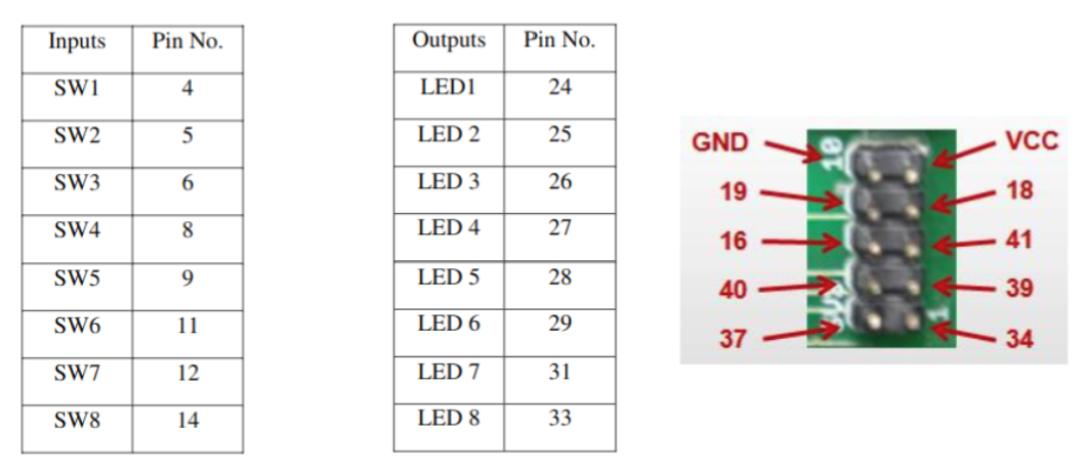
\includegraphics[width=0.52\textwidth]{figures/cpld_pinout.png}
        \caption{MAX3000A pinout for reference}
        \label{fig:circuitdiagram}
    \end{figure}

    \begin{table}[h!]
        \centering
        \begin{tabular}{|c|c|l|}
            \hline
            \textbf{Signal} & \textbf{Pin} & \textbf{Description} \\
            \hline
            clk & 43 & Global clock input (1Hz) \\
            o\_clk & 24 & Debugging clock output \\
            \hline
            bcd\_tens[3] & 34 & BCD tens place output (MSB) \\
            bcd\_tens[2] & 39 & BCD tens place output \\
            bcd\_tens[1] & 41 & BCD tens place output \\
            bcd\_tens[0] & 18 & BCD tens place output (LSB) \\
            bcd\_units[3] & 37 & BCD units place output (MSB) \\
            bcd\_units[2] & 40 & BCD units place output \\
            bcd\_units[1] & 16 & BCD units place output \\
            bcd\_units[0] & 19 & BCD units place output (LSB) \\
            \hline
            switch[7] (rst) & 14 & Reset signal input \\
            switch[6] & 12 & Switch input (bit 6) \\
            switch[5] & 11 & Switch input (bit 5) \\
            switch[4] & 9  & Switch input (bit 4) \\
            switch[3] & 8  & Switch input (bit 3) \\
            switch[2] & 6  & Switch input (bit 2) \\
            switch[1] & 5  & Switch input (bit 1) \\
            switch[0] & 4  & Switch input (bit 0) \\
            \hline
            led[6] & 33 & LED indicator (MSB) \\
            led[5] & 31 & LED indicator \\
            led[4] & 29 & LED indicator \\
            led[3] & 28 & LED indicator \\
            led[2] & 27 & LED indicator \\
            led[1] & 26 & LED indicator \\
            led[0] & 25 & LED indicator (LSB) \\
            \hline
        \end{tabular}
        \caption{Pin Mapping of MAX3000A as done in software}
        \label{tab:pinmapping}
    \end{table}
    
    \subsection{Truth Table and Circuit Diagram}
    
    The truth table and Circuit Diagram below outlines the system behavior during various phases of the game based on the cycle counter value:
    \vspace{15pt}
    \\
    Note - all the data are taken when seed phrase is 10101, for other seed the value will be different.

    \begin{table*}[tp]
        \centering
        \begin{tabular}{|c|c|c|c|}
            \hline
            \textbf{Cycle Counter} & \textbf{Action} & \textbf{Display Output} & \textbf{LED Status} \\
            \hline
            0-3 & Generate random number (LFSR) & Random value & Reflect LFSR value (padded) \\
            4 & Clear display & 0 & OFF \\
            5-10 & Accept user input via switches & Switch value & OFF \\
            11-12 & Display correct answer & Sum modulo 100 & LEDs ON (success or pattern) \\
            13-14 & Hold result display & Sum modulo 100 & LEDs remain in previous state \\
            15 & Reset game & 0 & LEDs ON \\
            \hline
        \end{tabular}
        \caption{Truth Table for Game Phases}
        \label{tab:truthtable}
    \end{table*}
    
    \begin{table*}[!t]
    \centering
        \begin{tabular}{|c|c|c|c|}
            \hline
            \textbf{Step} & \textbf{LFSR State (Binary)} & \textbf{Decimal Equivalent} & \textbf{Feedback (bit4 XOR bit2)} \\
            \hline
            0  & 10101 & 21 & 1 $\oplus$ 1 = 0 \\
            1  & 01010 & 10 & 0 $\oplus$ 0 = 0 \\
            2  & 10100 & 20 & 1 $\oplus$ 1 = 0 \\
            3  & 01000 & 8  & 0 $\oplus$ 0 = 0 \\
            4  & 10000 & 16 & 1 $\oplus$ 0 = 1 \\
            5  & 00001 & 1  & 0 $\oplus$ 0 = 0 \\
            6  & 00010 & 2  & 0 $\oplus$ 0 = 0 \\
            7  & 00100 & 4  & 0 $\oplus$ 1 = 1 \\
            8  & 01001 & 9  & 0 $\oplus$ 0 = 0 \\
            9  & 10010 & 18 & 1 $\oplus$ 0 = 1 \\
            10 & 00101 & 5  & 0 $\oplus$ 1 = 1 \\
            11 & 01011 & 11 & 0 $\oplus$ 0 = 0 \\
            12 & 10110 & 22 & 1 $\oplus$ 1 = 0 \\
            13 & 01100 & 12 & 0 $\oplus$ 1 = 1 \\
            14 & 11001 & 25 & 1 $\oplus$ 0 = 1 \\
            15 & 10011 & 19 & 1 $\oplus$ 0 = 1 \\
            16 & 00111 & 7  & 0 $\oplus$ 1 = 1 \\
            17 & 01111 & 15 & 0 $\oplus$ 1 = 1 \\
            18 & 11111 & 31 & 1 $\oplus$ 1 = 0 \\
            19 & 11110 & 30 & 1 $\oplus$ 1 = 0 \\
            20 & 11100 & 28 & 1 $\oplus$ 1 = 0 \\
            21 & 11000 & 24 & 1 $\oplus$ 0 = 1 \\
            22 & 10001 & 17 & 1 $\oplus$ 0 = 1 \\
            23 & 00011 & 3  & 0 $\oplus$ 0 = 0 \\
            24 & 00110 & 6  & 0 $\oplus$ 1 = 1 \\
            25 & 01101 & 13 & 0 $\oplus$ 1 = 1 \\
            26 & 11011 & 27 & 1 $\oplus$ 0 = 1 \\
            27 & 10111 & 23 & 1 $\oplus$ 1 = 0 \\
            28 & 01110 & 14 & 0 $\oplus$ 1 = 1 \\
            29 & 11101 & 29 & 1 $\oplus$ 1 = 0 \\
            30 & 11011 & 27 & 1 $\oplus$ 0 = 1 \\
            31 & 10111 & 23 & 1 $\oplus$ 1 = 0 \\
            \hline
        \end{tabular}
    \caption{Truth table showing the complete cycle of the 5-bit LFSR starting from 10101 as seed.}
    \end{table*}


    \begin{figure*}[!t]
        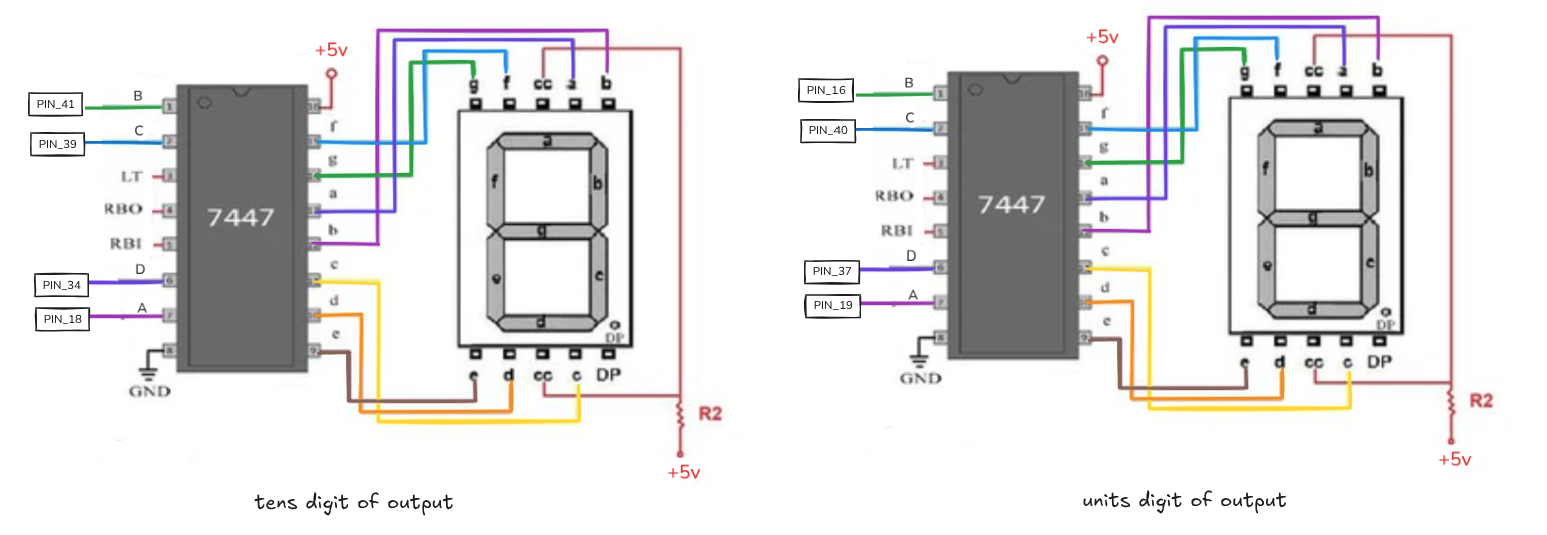
\includegraphics[width=.83\textwidth]{figures/circuit_diagram.png}
        \caption{CPLD Maths Game Circuit Diagram and IO Mapping}
        \label{fig:circuitdiagram}
    \end{figure*}
    
    \begin{figure*}[!t] 
        \centering
        \begin{subfigure}[b]{0.9\linewidth}
            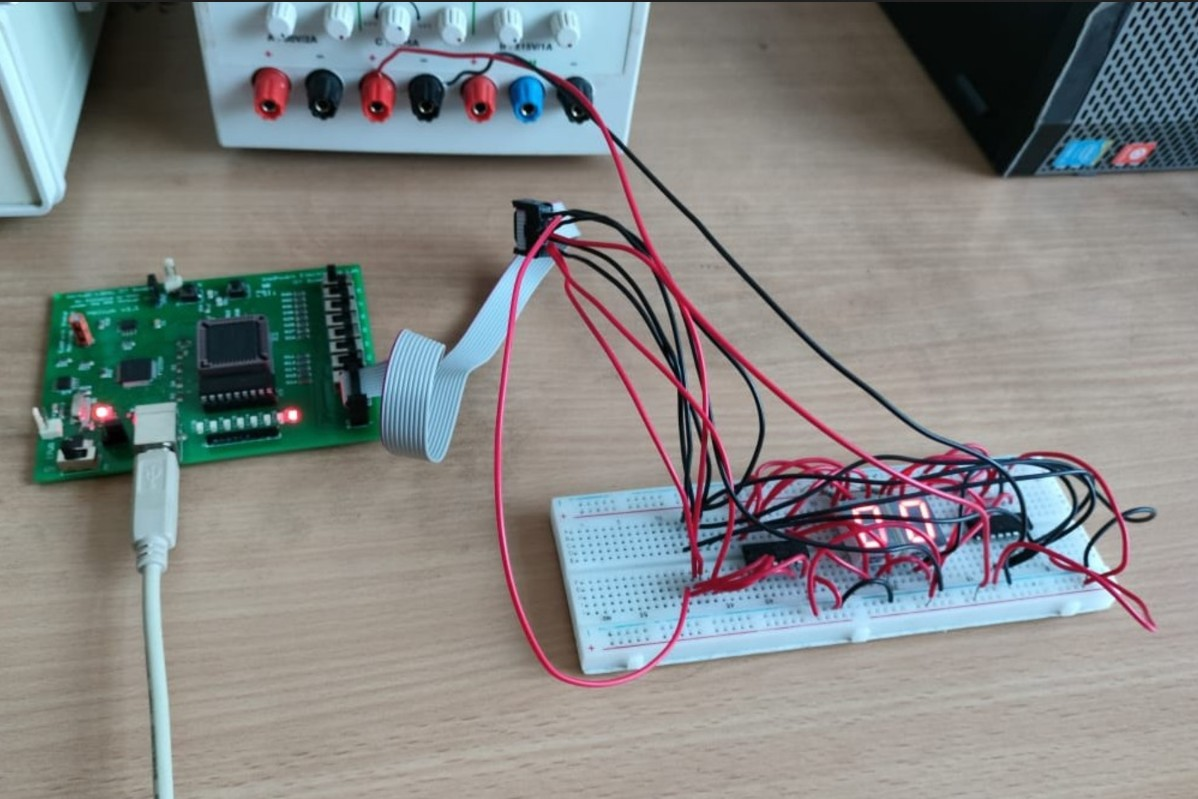
\includegraphics[width=\linewidth]{figures/ell201_proj_1.jpeg}
            \caption{Circuit connection CPLD and Breadboard used in the project}
            \label{fig:figa}
        \end{subfigure}
        \vspace{1cm}
        \begin{subfigure}[b]{0.9\linewidth}
            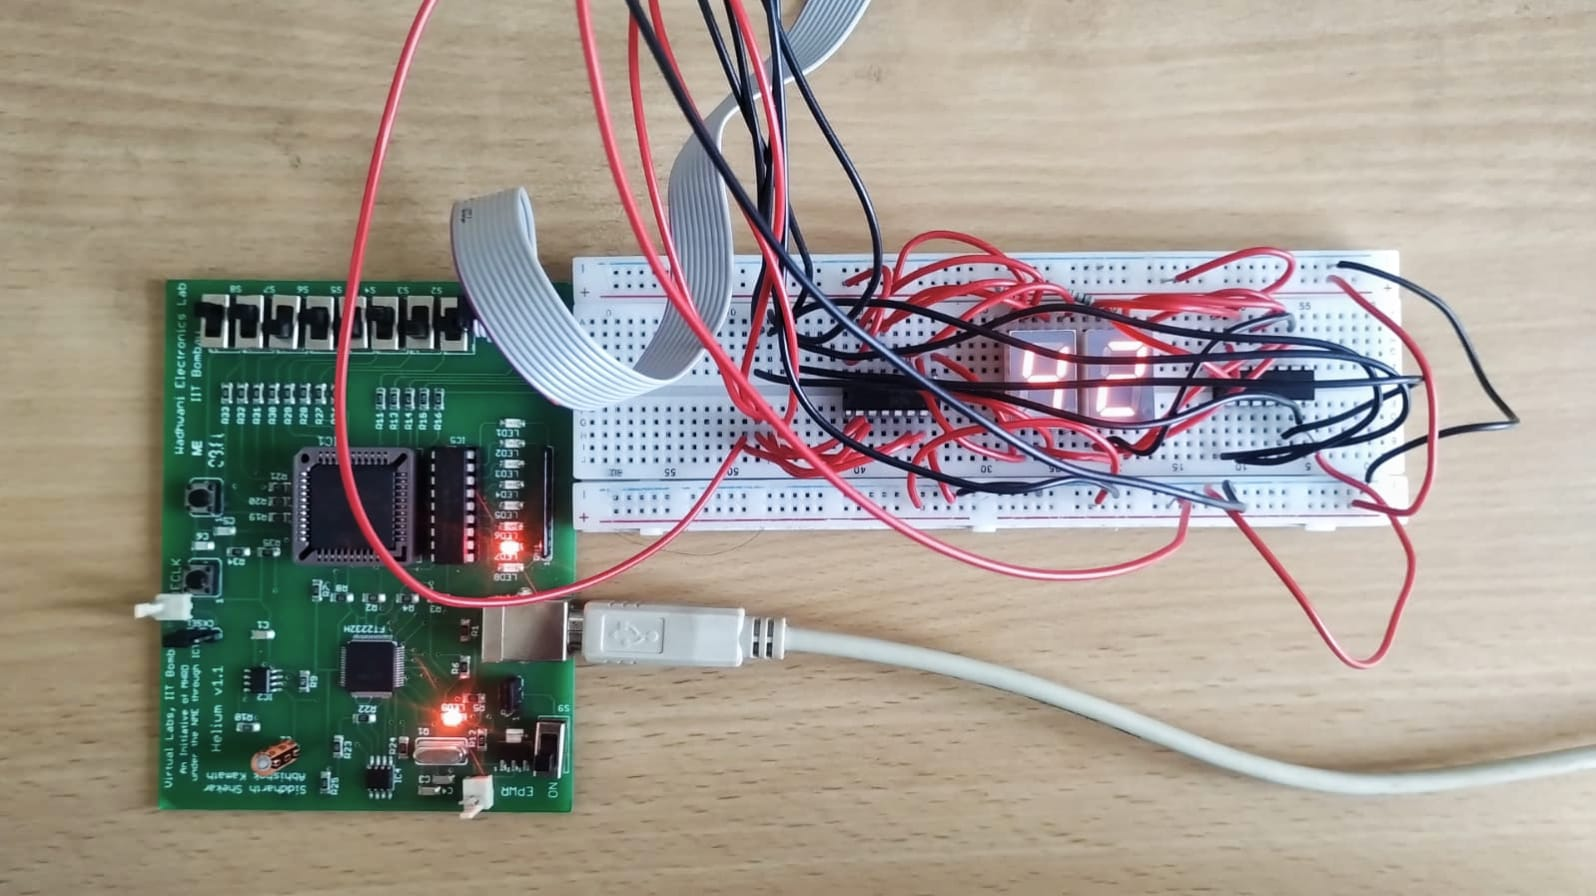
\includegraphics[width=\linewidth]{figures/ell201_proj_2.jpeg}
            \caption{Setup during Demonstration of project.}
            \label{fig:figb}
        \end{subfigure}
        \caption{CPLD demonstration}
        \label{fig:examplefloat}
    \end{figure*}


    \begin{figure*}[t]
    \centering
    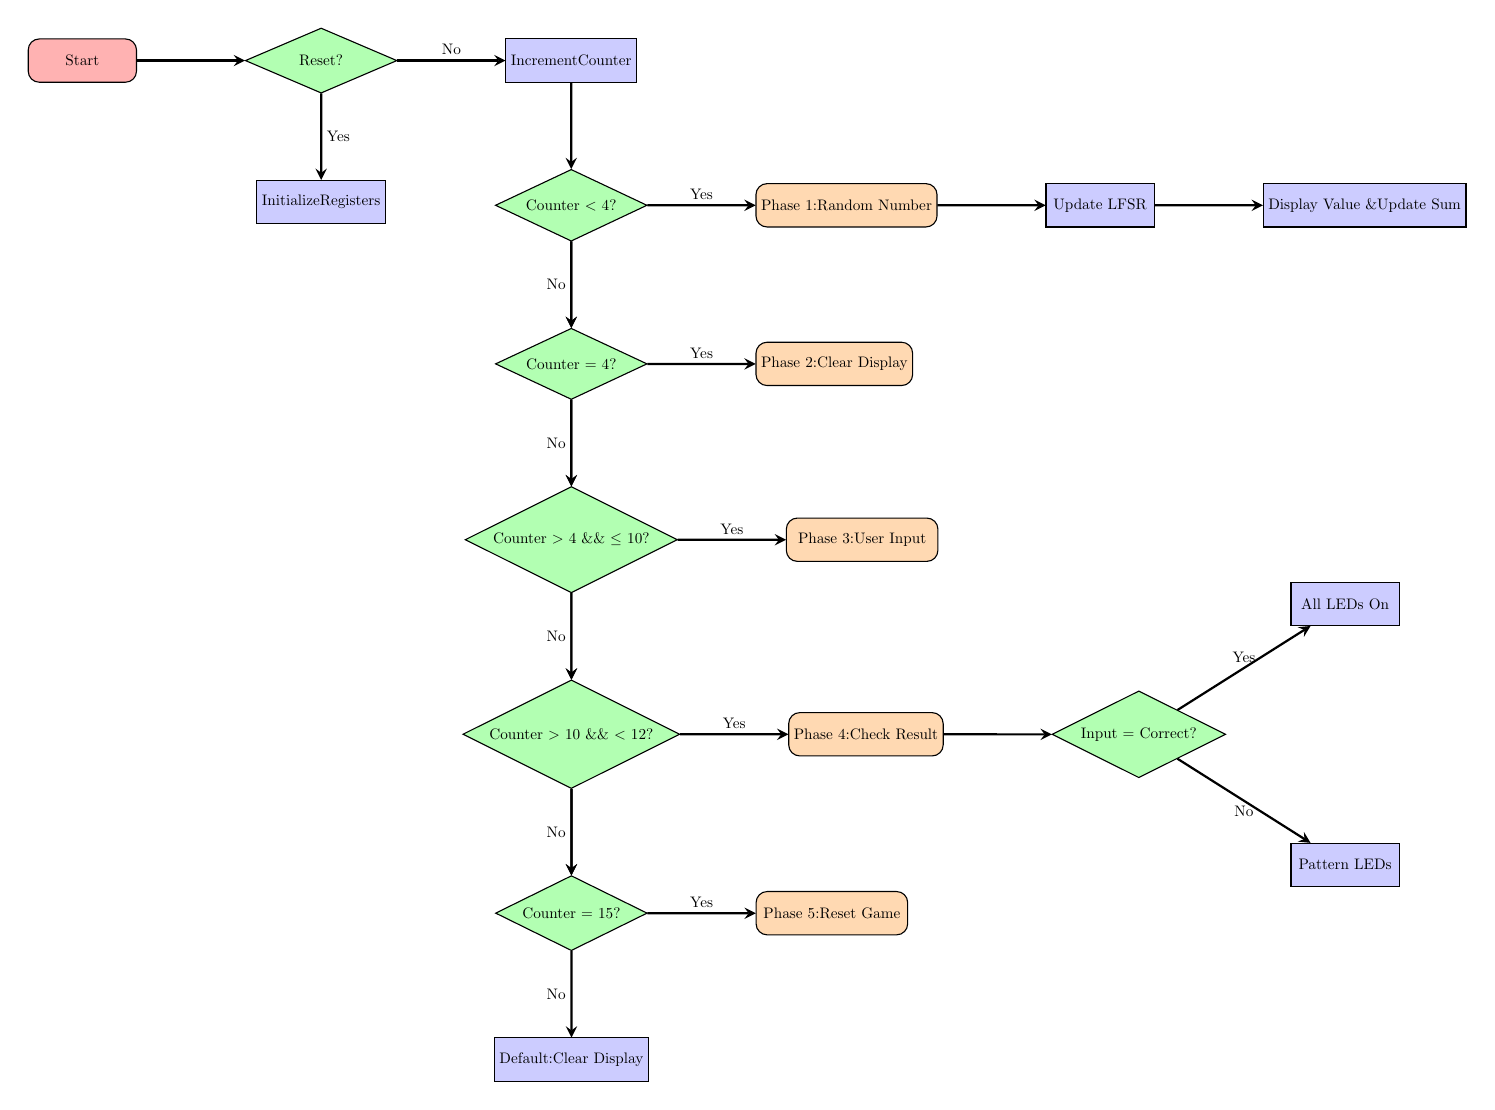
\begin{tikzpicture}[
        scale=0.55,
        transform shape,
        node distance=2cm and 2.5cm,
        startstop/.style={rectangle, rounded corners, minimum width=2.5cm, minimum height=1cm, text centered, draw=black, fill=red!30},
        process/.style={rectangle, minimum width=2.5cm, minimum height=1cm, text centered, draw=black, fill=blue!20},
        decision/.style={diamond, aspect=2, minimum width=3.5cm, minimum height=1.5cm, text centered, draw=black, fill=green!30},
        arrow/.style={thick,->,>=stealth},
        phase/.style={rectangle, rounded corners, minimum width=3.5cm, minimum height=1cm, text centered, draw=black, fill=orange!30},
    ]
        
        % Top row - start and initialization
        \node (start) [startstop] {Start};
        \node (reset) [decision, right=of start] {Reset?};
        \node (init) [process, below=of reset] {Initialize\\Registers};
        \node (increment) [process, right=of reset] {Increment\\Counter};
        
        % Main flow nodes in a grid
        % Row 1 - Phase 1
        \node (phase1check) [decision, below=of increment] {Counter \textless\ 4?};
        \node (phase1) [phase, right=of phase1check] {Phase 1:\\Random Number};
        \node (lfsr) [process, right=of phase1] {Update LFSR};
        \node (display) [process, right=of lfsr] {Display Value \&\\Update Sum};
        
        % Row 2 - Phase 2
        \node (phase2check) [decision, below=of phase1check] {Counter = 4?};
        \node (phase2) [phase, right=of phase2check] {Phase 2:\\Clear Display};
        
        % Row 3 - Phase 3
        \node (phase3check) [decision, below=of phase2check] {Counter \textgreater\ 4 \&\& $\leq$ 10?};
        \node (phase3) [phase, right=of phase3check] {Phase 3:\\User Input};
        
        % Row 4 - Phase 4
        \node (phase4check) [decision, below=of phase3check] {Counter \textgreater\ 10 \&\& \textless\ 12?};
        \node (phase4) [phase, right=of phase4check] {Phase 4:\\Check Result};
        \node (resultcheck) [decision, right=of phase4] {Input = Correct?};
        \node (correct) [process, above right=of resultcheck] {All LEDs On};
        \node (wrong) [process, below right=of resultcheck] {Pattern LEDs};
        
        % Row 5 - Phase 5
        \node (phase5check) [decision, below=of phase4check] {Counter = 15?};
        \node (phase5) [phase, right=of phase5check] {Phase 5:\\Reset Game};
        \node (default) [process, below=of phase5check] {Default:\\Clear Display};
        
        % Main flow connections - vertical spine
        \draw [arrow] (increment) -- (phase1check);
        \draw [arrow] (phase1check) -- (phase2check);
        \draw [arrow] (phase2check) -- (phase3check);
        \draw [arrow] (phase3check) -- (phase4check);
        \draw [arrow] (phase4check) -- (phase5check);
        
        % Start and reset connections
        \draw [arrow] (start) -- (reset);
        \draw [arrow] (reset) -- node[anchor=west] {Yes} (init);
        \draw [arrow] (reset) -- node[anchor=south] {No} (increment);
        % \draw [arrow] (init) -- ++(0,-1) -| (increment);
        
        % Feedback system - using a dedicated return path on the far left
        \coordinate (return) at ($(phase5check) + (-3,0)$);
        \coordinate (returntop) at ($(return) + (0,14)$);
        
        % Phase 1-5 horizontal connections
        \draw [arrow] (phase1check) -- node[anchor=south] {Yes} (phase1);
        \draw [arrow] (phase1) -- (lfsr);
        \draw [arrow] (lfsr) -- (display);
        
        \draw [arrow] (phase2check) -- node[anchor=south] {Yes} (phase2);
        \draw [arrow] (phase3check) -- node[anchor=south] {Yes} (phase3);
        
        \draw [arrow] (phase4check) -- node[anchor=south] {Yes} (phase4);
        \draw [arrow] (phase4) -- (resultcheck);
        \draw [arrow] (resultcheck) -- node[anchor=south] {Yes} (correct);
        \draw [arrow] (resultcheck) -- node[anchor=north] {No} (wrong);
        
        \draw [arrow] (phase5check) -- node[anchor=south] {Yes} (phase5);
        \draw [arrow] (phase5check) -- node[anchor=east] {No} (default);
        
        % Add "No" labels to remaining decisions
        \draw [arrow] (phase1check) -- node[anchor=east] {No} (phase2check);
        \draw [arrow] (phase2check) -- node[anchor=east] {No} (phase3check);
        \draw [arrow] (phase3check) -- node[anchor=east] {No} (phase4check);
        \draw [arrow] (phase4check) -- node[anchor=east] {No} (phase5check);
    \end{tikzpicture}
    \caption{Control flow diagram for the CPLD Maths Game implementation}
    \label{fig:controlflow}
    \end{figure*}


		
\section{Finite State Machine (FSM) Design}

The core control logic of the system is implemented using a synchronous Finite State Machine (FSM), which sequences through distinct operational phases of the arithmetic game. The FSM operates based on a classical Mealy-style structure that includes both present-state and next-state logic, as commonly recommended in structured Verilog designs. 

The FSM transitions through the following states:

\begin{itemize}
    \item \textbf{IDLE} – Initial state; waits for system reset or start condition.
    \item \textbf{GENERATE} – Activates a 5-bit Linear Feedback Shift Register (LFSR) to generate a sequence of pseudo-random numbers. The LFSR, being a maximal-length feedback register, cycles through $2^5 - 1 = 31$ unique non-zero states \cite{nandland_lfsr}.
    \item \textbf{DISPLAY} – Sequentially outputs generated numbers to the 7-segment display. Internally, a running sum is updated synchronously.
    \item \textbf{INPUT} – Accepts user input through DIP switches; values are latched using synchronous sampling techniques.
    \item \textbf{CHECK} – Compares the stored sum with the player’s input. Non-blocking assignments ensure correct state progression.
    \item \textbf{FEEDBACK} – Drives LED outputs to indicate correctness and resets the FSM after a brief delay.
\end{itemize}

All transitions are driven by a 1Hz system clock. The FSM design adheres to synchronous logic principles and uses non-blocking assignments (`<=`) to avoid race conditions. Debouncing is handled externally or assumed negligible due to clock throttling.



\section{Linear Feedback Shift Register (LFSR) Logic}

In this project, a 5-bit Linear Feedback Shift Register (LFSR) is employed as a hardware-based pseudo-random number generator (PRNG) to introduce non-determinism into the arithmetic memory game. The LFSR operates synchronously with the system clock and updates its state on every positive clock edge.

The implemented LFSR uses a primitive characteristic polynomial of the form:

\begin{equation}
    P(x) = x^5 + x^3 + 1
\end{equation}

This corresponds to feedback taps at bit positions 4 and 2 (0-indexed), generating a maximal-length sequence of $2^5 - 1 = 31$ non-zero states before repetition. The feedback logic for the next input bit is given by:

\begin{equation} \label{eq:lfsr}
    \texttt{next\_bit} = \texttt{lfsr}[4] \oplus \texttt{lfsr}[2]
\end{equation}

At each clock cycle, the current LFSR state undergoes a right-shift operation, with \texttt{next\_bit} injected into the most significant bit (MSB). The resulting sequence ensures that the game remains challenging and memory-driven.

The design is fully synchronous and avoids the use of blocking assignments, preserving timing determinism across state updates. The LFSR is reset asynchronously to a non-zero seed value. This implementation ensures compliance with standard digital PRNG design principles.



    


\section{Test Bench Waveforms}

\begin{figure*}[!t]
    \centering
    \begin{subfigure}[b]{0.9\textwidth}
        \centering
        \includegraphics[width=\linewidth]{figures/tb_gmp1.jpg}
        \caption{Testbench waveform output (Part 1).}
        \label{fig:tb_part1}
    \end{subfigure}
    \vspace{1em}
    \begin{subfigure}[b]{0.9\textwidth}
        \centering
        \includegraphics[width=\linewidth]{figures/tb_gmp2.jpg}
        \caption{Testbench waveform output (Part 2).}
        \label{fig:tb_part2}
    \end{subfigure}
    \caption{Combined simulation waveforms showing the DUT behavior over two capture windows.}
    \label{fig:tb_waveforms}
\end{figure*}
 \lstinputlisting[caption=Verilog code, language=Verilog,label=code]{tb_gmp.v}

	
\section{Verilog codes}
	
    \lstinputlisting[caption=Verilog code, language=Verilog,label=code]{gmp.v}
	



\section{Future Improvements}

Several enhancements can be incorporated to expand the functionality and interactivity of the current system:

\begin{enumerate}
    \item \textbf{Random Seed:} 
    Currently, the LFSR uses a hardcoded seed (\texttt{10101}) for pseudo-random number generation. A future improvement could allow the user to input a 5-bit seed value through switches, making each game session more unpredictable and engaging. This feature was not implemented due to hardware resource constraints (63 out of 64 macrocells were already utilized).
    \begin{figure}[h!]
        \centering
        \includegraphics[width=0.4\textwidth]{figures/issue_marcoshells.png}
        \caption{exceeding macroshells 72/64 when trying to extend its capability.}
        \label{fig:circuitdiagram}
    \end{figure}

    \item \textbf{Difficulty Levels:}
    Adding levels of increasing difficulty, such as displaying more numbers or introducing subtraction/multiplication could make the game more challenging and educational.
    

    \item \textbf{Score Display:}
    Enhancing the system to retain and display the player's score over multiple rounds would improve game continuity and user engagement.

\end{enumerate}

\section{Conclusion}

This project demonstrates the application of Verilog HDL and CPLD-based digital design principles to build an interactive and educational arithmetic memory game. By combining modular FSM-based control logic, pseudo-random number generation through LFSR, and real-time user interaction using switches and displays, we were able to deliver a robust embedded system. The game not only tests a player's arithmetic skills but also offers immediate feedback, reinforcing user engagement.

Through this implementation, we deepened our understanding of digital logic, timing constraints, and hardware debugging using the MAX3000A platform. The project serves as a foundation for more sophisticated embedded applications involving gamified learning or educational electronics. Future iterations could explore porting the design to FPGAs or integrating soft-core processors for extended functionality.

\section{Acknowledgements}

We would like to express our sincere gratitude to our Teaching Assistant, Chithambara J, for their continuous support and insightful feedback throughout the semester. Their guidance was immensely helpful in enhancing our technical understanding and in fostering a deeper interest in digital system design and embedded applications.

\vspace{2em}
\begin{center}
  \large\textbf{-----------  Thank You  -----------}
\end{center}

%----------------------------------------------------------

\end{document}